\noindent
The application of Generative AI has shifted significantly between the two main phases of the project. 

\noindent
While in the RASD phase, models were primarily used for translating textual use cases into high-fidelity UI mockups, in the DD, the focus moved towards textual reliability and technical precision.

\noindent
In this phase, Google Gemini was not used to invent features, but rather to act as a rigorous technical writer. The primary goal was to ensure that the written documentation perfectly matched the architectural decisions made by the team.
\subsection{Example of Interaction: Publish Path Sequence Diagram Description}

The following examples illustrate the practical interaction with Gemini used to draft the documentation. In this workflow, the Sequence Diagrams were uploaded as visual inputs; the model analyzed the architectural logic depicted in the images and generated the corresponding textual descriptions presented in this document.

\vspace{0.3cm}
\begin{PromptBox}
\quad Give me a short description of this sequence diagram

\textbf{} \\
    \begin{center}
    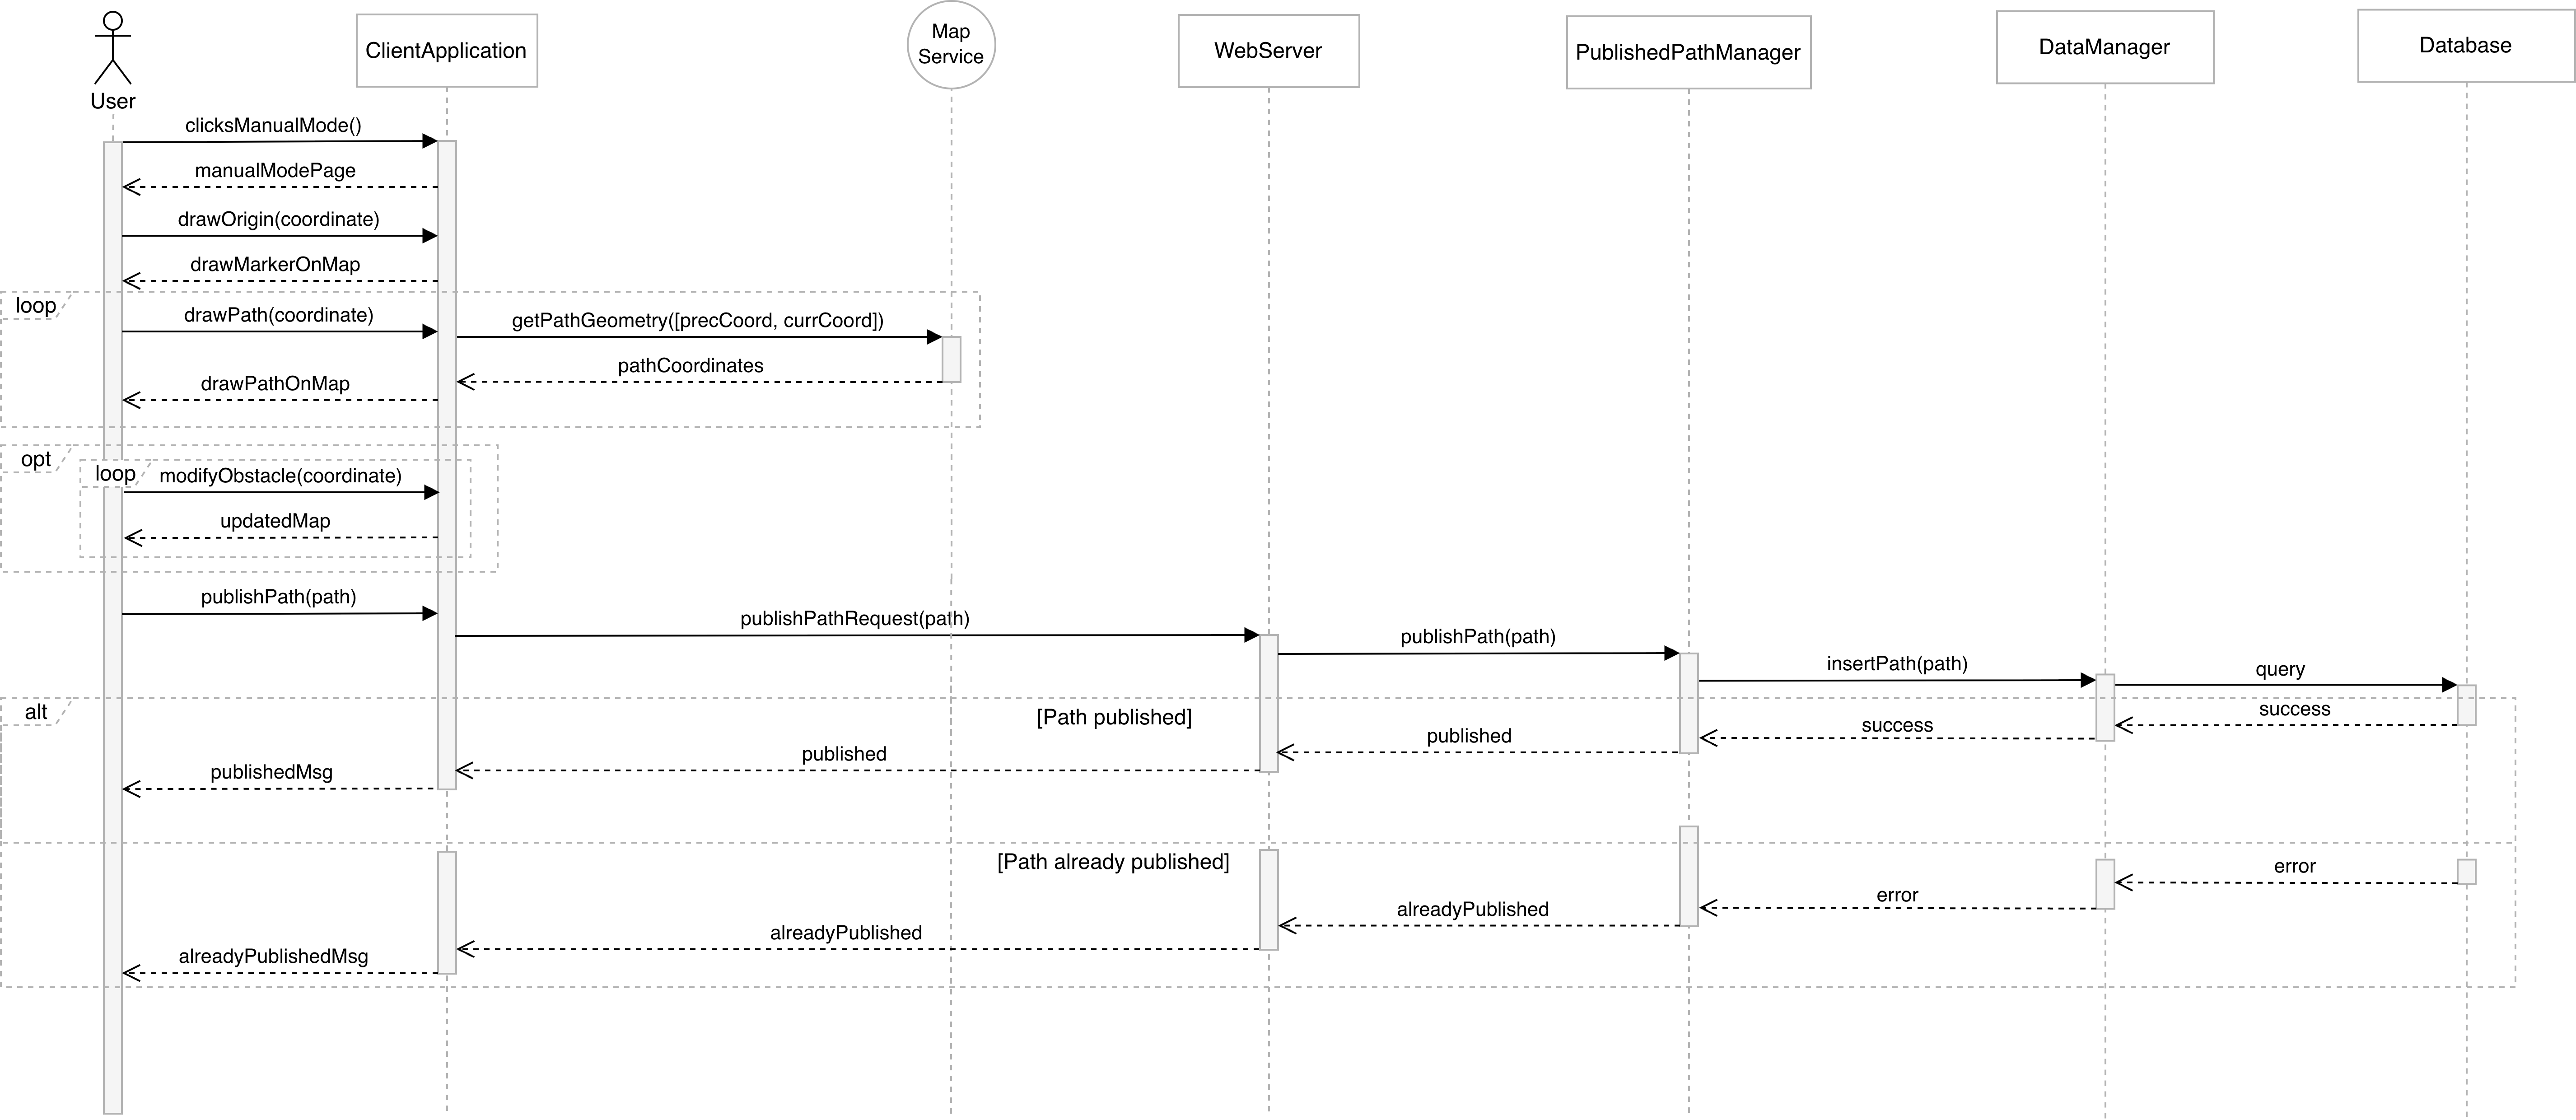
\includegraphics[height=5.5cm, keepaspectratio]{DD/Images/SequenceDiagram/PublishPath.png}
    \end{center}
    
\vspace{0.3cm}

\vspace{0.3cm}
\end{PromptBox}


\begin{GeminiGood}
\quad The User activates manual mode from the ClientApplication, which displays the dedicated page and allows the user to draw the origin and the path directly on the map. During the drawing phase (the loop block), the client requests the path geometry from the WebServer; the request is forwarded to the PublishedPathManager, which queries the Map Service through the Proxy to obtain the correct path coordinates, which are then displayed on the map.

Optionally (the opt block), the user can modify obstacles along the path, updating the map in real time.

When the user decides to publish the path, the client sends a publishPath request to the server. In the alt block:

If the path has not been published yet, the DataManager stores it in the Database, the operation succeeds, and the user receives a confirmation message.

If the path has already been published, an error is returned and the client shows a “path already published” message.

The diagram highlights the complete flow of path drawing, validation, and publication


    
\vspace{0.3cm}

\end{GeminiGood}

\vspace{0.5cm}



\noindent
The textual descriptions generated by Gemini accurately captured the logical flow and the sequence of messages depicted in the diagrams. However, these outputs were utilized primarily as initial drafts.
\noindent
The development team subsequently reviewed and reworked the content independently to ensure it perfectly aligned with the specific design nuances. The AI was leveraged mainly to establish a high standard of English technical writing and grammatical correctness, acting as an advanced drafting assistant rather than an autonomous author.

\subsection{Conclusion}
Although Gemini significantly accelerated the drafting phase, the final responsibility for the accuracy of the system specifications lies entirely with the development team. Every line of text was manually verified to strictly adhere to the project's requirements.
